\documentclass[11pt, a4paper]{article}
\usepackage[utf8]{inputenc}
\usepackage{graphicx}
\usepackage{setspace}
\usepackage{array}
\usepackage{fancyhdr}
\usepackage[none]{hyphenat}
\usepackage{rotating}
\usepackage{anyfontsize}
% For subfigures
\usepackage{caption}
\usepackage{subcaption}
% Get rid of the indent of the first line
\edef\restoreparindent{\parindent=\the\parindent\relax}
\usepackage{parskip}
% Fix text out of margin
\emergencystretch 3em
% Set date format
\usepackage[ddmmyyyy]{datetime}
% Set fonts
\usepackage{fontspec}
\setmainfont{Muli}[
    Path = fonts/ ,
    Extension = .ttf ,
    UprightFont = *-Regular ,
    ItalicFont = *-Italic ,
    BoldFont = *-Bold ,
    BoldItalicFont = *-BoldItalic
]
\setsansfont{Muli-Black}[
    Path = fonts/ ,
    Extension = .ttf ,
    ItalicFont = *Italic
]
% Set page margin
\usepackage{geometry}
\geometry{a4paper,
            % total={175mm,257mm}, %space for content
            headheight=80pt,
            headsep=2pt,
            % top=3cm,
            bottom=2.5cm,
            left=2cm,
            right=1.75cm}
% Set the name of the table of contents
\usepackage{url}                                                  % for correct typesettings of URLs
\usepackage{hyperref}                                             % for sophisticated linking of urls, dois, pictures, tables, etc.
\hypersetup{
    unicode=true,                                                 % non-Latin characters in Acrobat’s bookmarks
    pdftoolbar=true,                                              % show Acrobat’s toolbar?
    pdfmenubar=true,                                              % show Acrobat’s menu?
    pdffitwindow=false,                                           % window fit to page when opened
    pdfstartview={FitH},                                          % fits the width of the page to the window
    pdfauthor={C. Fortmann-Grote},                                           % author
    pdftitle={MS5.3: VINYL Software Release},   % title
    pdfsubject={PaNOSC WP5 (ViNYL) Milestone MS5.3},                             % subject of the document
    pdfcreator={pdflatex},                                         % creator of the document
    pdfnewwindow=true,                                            % links in new PDF window
    colorlinks=true,                                              % false: boxed links; true: colored links
    linkcolor=black,                                                % color of internal links (change box color with linkbordercolor)
    citecolor=blue,                                                % color of links to bibliography
    filecolor=blue,                                               % color of file links
    urlcolor=blue                                                 % color of external links
}
% \usepackage[style=nature]{biblatex}
% \addbibresource{references.bib}



\pagestyle{fancy}
\fancyhead{} % clear all header fields
\fancyfoot{} % clear all footer fields
\renewcommand{\headrulewidth}{0pt} % clear the header ruler line
\setlength{\footskip}{14pt}
\fancyfoot{} % clear all footer fields
\fancyfoot[R]{\hspace{1em}}
% \fancyfoot[c]{\begin{tabular}{c}
% 
\includegraphics[width=\textwidth, valign=b]{footer.pdf}& \\
% \end{tabular}}
\fancyfoot[L]{\hspace{1cm} 
\includegraphics[width=0.95\textwidth]{footer.pdf}}
% \cfoot{
\includegraphics[width=0.95\textwidth]{footer.pdf}}

% Set line spacing
\emergencystretch 3em
\setstretch{1.2}
% \setlength{\footskip}{10pt}

\begin{document}
% \thispagestyle{empty}
\chead{
\includegraphics[width=\textwidth]{header.pdf}}

{
	\centering
    \begin{onehalfspace}
    \sffamily
     \vspace*{5ex}
	{\fontsize{20}{24}\selectfont PaNOSC \par}
	{\fontsize{20}{24}\selectfont Photon and Neutron Open Science Cloud \par}
	{\fontsize{20}{24}\selectfont H2020-INFRAEOSC-04-2018 \par}
	{\fontsize{20}{24}\selectfont Grant Agreement Number: 823852 \par}
	\end{onehalfspace}

	\vspace*{7ex}
	
\includegraphics[width=\textwidth]{PaNOSClogo_web_RGB.pdf}\par
	\vfill
	{\large \textbf{\sffamily MS5.3: VINYL Software Release}}\par
} % end of centering


\includegraphics[width=1.27in]{by.eps}\par
This work is licensed under a Creative Commons Attribution 4.0 International License\\
(\url{http://creativecommons.org/licenses/by/4.0/})\par

% \vspace*{0ex}
\newpage

% Set footer for the second page
% \setlength{\footnotesep}{50pt}
% \setlength{\footskip}{0pt}
\fancyfoot{} % clear all footer fields
\fancyfoot[R]{\thepage}
% \fancyfoot[c]{\begin{tabular}{c}
% 
\includegraphics[width=\textwidth, valign=b]{footer.pdf}& \\
% \end{tabular}}
\fancyfoot[L]{\hspace{1cm} 
\includegraphics[width=0.95\textwidth]{footer.pdf}}


{ %Front page
\restoreparindent
% \renewcommand{\arraystretch}{1.2} % change table row height

{\sffamily\huge Project Deliverable Information Sheet \par}

\begin{center}
\begin{tabular}{ | m{5.2cm}| m{10.7cm} | }
\hline
Project Reference No. & 823852 \\
\hline
Project acronym: & PaNOSC \\
\hline
Project full name: & Photon and Neutron Open Science Cloud \\
\hline
H2020 Call: & INFRAEOSC-04-2018 \\
\hline
Project Coordinator: & Andy Götz (andy.gotz@esrf.fr) \\
\hline
Coordinating Organization: & ESRF \\
\hline
Project Website: & www.panosc.eu \\
\hline
Deliverable No: & MS5.3: VINYL Software Release\\
\hline
Deliverable Type: & Software \\
\hline
Dissemination Level: & Public \\
\hline
Contractual Delivery Date: & 30/05/2022 \\
\hline
Actual Delivery Date: & \today \\
\hline
EC project Officer: & Ren\'e Martins \\
\hline
\end{tabular}
\end{center}

{\large \textbf{Document Control Sheet} \par}
\begin{center}
\begin{tabular}{ | m{5.2cm}| @{}c@{} | }
\hline
\textbf{Document}
&
\begin{tabular}{| m{10.7cm} |}
Title: MS5.3: VINYL Software Release \\\hline
Version: 1 \\\hline
Available at: \\\hline
Files: 1 \\\hline
\end{tabular}
\tabularnewline\hline
\textbf{Authorship}
&
\begin{tabular}{| m{10.7cm} |}
Written by: Carsten Fortmann-Grote \\\hline
Contributors:   Mads Bertelsen,
Stella d'Ambrumenil,
Juncheng E,
Aljo\v{s}a Hafner,
Gergely Norbert Nagy,
Shervin Nourbakhsh,
Mousumi Upadhyay Kahaly \\\hline
Reviewed by: Jordi Bodera Sempere\\\hline
Approved:  Andy Götz\\\hline
\end{tabular}
\tabularnewline\hline
\end{tabular}
\end{center}

{\large \textbf{List of participants} \par}
\begin{center}
    \begin{tabular}{|m{3.0cm}|m{9.5cm}|m{3cm}|}
        \hline
        \textbf{Participant No.} & \textbf{Participant organisation name} & \textbf{Country} \\
        \hline
        1 & European Synchrotron Radiation Facility (ESRF) & France \\
        \hline
        2 & Institut Laue-Langevin (ILL) & France \\
        \hline
        3 & European XFEL (XFEL.EU) & Germany \\
        \hline
        4 & The European Spallation Source (ESS) & Sweden \\
        \hline
        5 & Extreme Light Infrastructure Delivery Consortium (ELI-DC) & Belgium \\
        \hline
        6 & Central European Research Infrastructure Consortium (CERIC-ERIC) & Italy \\
        \hline
        7 & EGI Foundation (EGI.eu) & The Netherlands \\
        \hline
    \end{tabular}
\end{center}

}%End front page

% Table of contents
\newpage
\addtocontents{toc}{\protect\thispagestyle{fancy}}
\newpage
\tableofcontents
\newpage
% End Table of contents

\section{Introduction}
The design and
implementation of a user interface (UI) requires special attention in any
software product. A simulation software package must expose interfaces for
the configuration of the simulation task, provision of input data, execution of
the task including task and data distribution on parallel compute architectures,
data retrieval and documentation. Traditionally, each simulation
package implements its own specialized user interface making it hard for users
to learn the usage of multiple different simulation tools.
Furthermore, simulation pipelines that concatenate various simulation steps have to provide wrappers for each
 simulation in the pipeline. Our python3 package \textit{libpyvinyl} addresses
these issues by providing a base software layer that supports the aforementioned
user interface functionalities in a generic way and ontop of which simulation
codes and simulation frameworks\footnote{By `framework', we
  understand a software product that supports configuration, execution and data
  retrieval
  for one or several simulation codes but that does not necessarily implement a
  simulation algorithm itself, rather, it drives simulations based on the user's
  input. An example would be the Oasys project, a framework for x-ray optics
  simulations.} can build their specialized implementations. We strive to
abstract away as much as possible the details of user interface functionalities
while
maintaining enough flexibility to support implementation of truly new functionality.

Simulation packages built on \textit{libpyvinyl} will be
able to skip basic tasks on parameters and software structure and go straight
to implementing interesting scattering physics. Furthermore such packages
will adhere to a standard scheme, facilitating collaboration across
different simulation codes that share \textit{libpyvinyl} as a foundation.
The most crucial benefit is
however that users will find the interfaces of packages built on
\textit{libpyvinyl} similar and thus what they learn using one package will be
transferable to the others. These are the benefits of standardisation and
harmonisation. The SimEx and McStasScript packages that simulate X-ray and
Neutron instruments, respectively have  already adopted \textit{libpyvinyl}.

In the following, this report documents the components of \textit{libpyvinyl}, their
relation to each other as well as the installation and utilization of the
package. \textit{libpyvinyl} is registered on zenodo at \url{https://dx.doi.org/10.5281/zenodo.6558164}. At the time of writing, the latest release is version v1.1.1. 

\section{Libpyvinyl and its components}
\label{sec:libpyvinyl}
Since \textit{libpyvinyl} needs to serve as a flexible foundation, it is
important that the layout is general. The overall structure is briefly outlined
here before the major components are described in their separate sections.

The basic unit in a simulation is referred to as a \textit{Calculator} as it
represents the execution of a simulation algorithm.
Specification of the required input parameters and input data as well as the
output data is the developer's responsibility. The \textit{Data} class
represents input and output data while the \textit{Parameters} class represents
simulation configuration parameters. These software entities already support a
number of use cases including the concatenation of simulation steps where output
data from one \textit{Calculator} becomes the input of the next
\textit{Calculator}.
Such a simulation pipeline is represented by the \textit{Instrument} class.

\subsection{Calculators}
\label{sec:calculators}
The calculator is a very general class that can take input and can provide
output. All code that affect the physics of the simulation is contained within
such calculators, it could for example be a calculator for a piece of optics or
a sample. The input of a calculator can be data in the form of one or more data
objects \ref{sec:data} and a input for a number of parameters
\ref{sec:parameters}. The output is also organised as data objects. When a new
calculator is developed, the dependence on the external data and parameters is
specified. Figure~\ref{fig:libpyvinyl_classes_schema} gives a schematic
representation of these base classes and some specialized classes. 


\begin{figure}[ht]
  \centering
  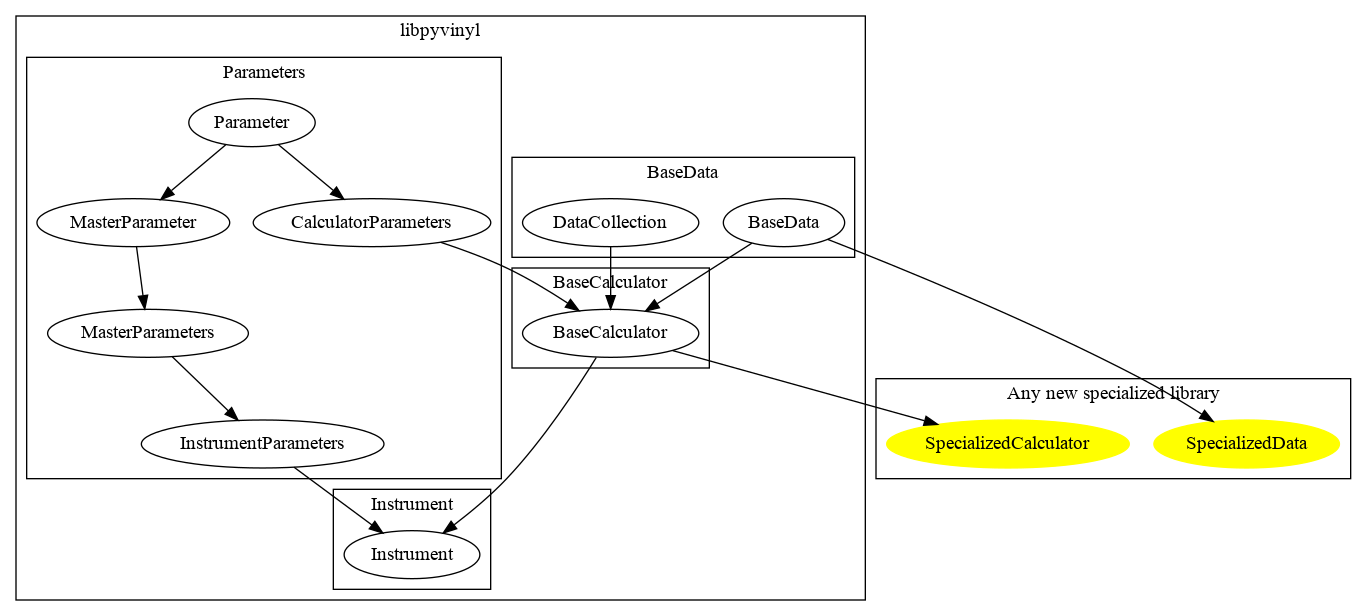
\includegraphics[width=.8\textwidth]{figures/libpyvinyl_classes_relations.png}
  \caption[\textit{libpyvinyl} schema]{Schematic representation of the
    \textit{libpyvinyl} base classes, derived classes and their role in
    describing complex simulation pipelines. Highlighted classes are implemented
  by specialized simulation software developers. These inherit the generic
  functionality and entity relations from \textit{libpyvinyl}'s base and derived classes.}
  \label{fig:libpyvinyl_classes_schema}
\end{figure}

\subsection{Data}
\label{sec:data}
The \textit{libpyvinyl} package provides baseclasses for both individual
datasets, the \textit{Data} class (e.g. to represent a single simulated diffraction image)
as well as  collections of datasets (a series of diffraction images from
 sequential sample exposures). These objects  mainly facilitate the data transfer between \textit{Calculators}.

\subsection{Parameters}
\label{sec:parameters}
The individual parameters are usually defined by a calculator class using the
\textit{libpyvinyl} base parameter class. This class includes the ability to
contain arrays, units and permissible value ranges. The \textit{Parameters}
class is a major part of the safety net that prevents a user from faulty
configuration of the interfaced simulation code which would cause runtime
errors or lead to wrong or misleading results.

\subsection{Instruments}
\label{sec:instruments}
Instruments are conceptually a series of \textit{Calculators} but can also contain 
master parameters that configure the simulation globally.
One could imagine a source \textit{Calculator}, some optics
\textit{Calculators}, a sample \textit{Calculator} and then a detector \textit{Calculator} along with a
\textit{Parameter} describing the simulated energy. As a \textit{MasterParameter}, information
about the simulated energy can be provided to multiple \textit{Calculators} that would
need that information to avoid the user having to specify redundant information.
The chain of \textit{Calculators} can then be executed by calling the
\textit{Instrument}'s member functions.

\section{Software availability and Installation}
\label{sec:installation}
The source code for \textit{libpyvinyl} is hosted on github.
Tagged releases are registered 
the python package index \textit{pypi} as documented in Sec.~\ref{sec:pypi}.

Each commit to the code base triggers a build--test--deploy cycle. 
Besides building the library components, also the documentation is compiled
and published. Table~\ref{tab:links} provides the URLs to the aforementioned
resources.

\begin{table}[ht]
  \centering
  \begin{tabular}{l|l}
 Software repository &   \url{https://github.com/PaNOSC-ViNYL/libpyvinyl} \\
 Releases registry &   \url{https://github.com/PaNOSC-ViNYL/libpyvinyl/releases} \\
 Pypi & \url{https://pypi.org/libpyvinyl} \\
 CI/CD status &   \url{https://github.com/PaNOSC-ViNYL/libpyvinyl/actions} \\
 Documentation &    \url{https://libpyvinyl.readthedocs.io/}
  \end{tabular}
  \caption{Resource URLs for \textit{libpyvinyl}}
  \label{tab:links}
\end{table}
 

\subsection{Dependencies and requirements}
\label{sec:dep}

\textit{libpyvinyl} is continuously tested on python versions 3.6 until 3.10.
Required python packages are listed in the repository's \textit{requirements}
files and will be installed automatically if the following instructions are applied.

\subsection{Installation from the python package index pypi}
\label{sec:pypi}

Installation via \textit{pypi} is the most straightforward method. On a Unix based
system, the shell command
\begin{verbatim}
$> pip install libpyvinyl
\end{verbatim}
will download, configure, and install the library into the users current python
runtime environment.

\subsection{Installation from source}
\label{sec:source}

Installing the library directly from the sources allows to install the latest,
potentially unstable, release. This may be an option for developers seeking to
contribute to \textit{libpyvinyl} or to test new features that are not available
in the released versions yet.

To get the sources from github and then install into the current runtime environment:
\begin{verbatim}
$> git clone https://github.com/PaNOSC-ViNYL/libpyvinyl
$> pip install [-e] .
\end{verbatim}
Activating the option \texttt{-e} will link the installed code to the downloaded
sources such that changes in the source code would immediately be reflected in
the runtime environment, i.e. no re-installation is required.

\section{Instructions for developers}
\label{sec:dev}
Extensive usage instructions for developers of downstream simulation codes are
provided in the online documentation. Here we only summarize the main points:
\begin{description}
\item[Identify needed components] Not all components provided by
  \textit{libpyvinyl} may be needed to implement the targeted functionality.
  E.g. a standalone simulation code does not necessarily have to implement the
  \textit{Instrument} class functionalities.
 
\item[Inherit base classes] In their simulation code, developers would then
  define their own classes to represent data, code execution, parameters etc.
  Fig.~\ref{fig:libpyvinyl_classes_schema} hints at which classes to inherit
  from for the various components.

 
\item[Implement specialized functionality] In many cases, only a very limited
  number of methods need to be implemented and members declared. Consult the
  source code of each parent class as well as the examples provided in the
  documentation.

 
\item[Test] We strongly recommend to add unit and regression tests for your
  derived classes. Examples for how to setup a test class are provided in the
  \texttt{tests/} directory of the source code repository. In particular,
  \texttt{tests/integration/plusminus} contains tests for a derived
  \textit{Calculator} which is also documented as an example in the documentation.
  
\end{description}

% \fancypagestyle{plain}{}

\end{document}
